\begin{appendix}

{\Large \bf Appendix}
\appendix

\section{Details in creating $\delta$ for input independence}
The additional regularization terms in the loss function for creating $\delta$ for input independence test is as follows:
$$ \pazocal{R} = \eta_2\big[(x + \delta - p_{h})^+ + (p_{l} - x - \delta)^+\big] + \eta_3\sum{\delta \odot (J - I_c)}$$
$\eta_2\big[(x + \delta - p_{h})^+ + (p_{l} - x - \delta)^+\big]$ penalizes pixel values in $x+\delta$ that fall outside the valid pixel range $[p_{\textit{l}}, p_{\textit{h}}]$ (e.g., $[0, 255]$). The additional term $\eta_3\sum{\delta \odot (J - I_c)}$ minimizes updates to regions outside of the $\delta$ region represented by mask $I_c$ ($J$ is a matrix of ones). The overall loss function is:
$$L = \|f(x+\delta)-f(x)\|_2 - \eta_1\|\delta\|_2 + \pazocal{R}$$
The update rule for $\delta$ is:
$$\delta_{t+1} = \delta_t - \lambda \frac{\partial L}{\partial \delta}$$
where $\lambda$ is the step size (defaults to $500$). $\delta_0$ is initialized from a dog image to obtain solutions that are semantically meaningful.

\section{Discussions on $\delta$ versus common feature}
Note that there is a subtle difference between $\delta$ generated from the optimization procedure above versus the common feature (\CF) obtained from training. Intuitively, to find $\delta$, we are moving an input in the direction perpendicular to $\nabla_xf(x)$, but the gradient itself is fixed because the model is fixed. When training a model with \CF, $\nabla_xf(x)$ becomes small with respect to the \CF. This explains why we expect minimal attribution change when $\delta$ is added to the input during input independence testing, but expect small attribution to dog \CF~during input dependence testing.

\section{Other measures for input independence}
An alternative measure of input independence is the average attribution difference when $\delta$ is added to the input:
$$\frac{1}{|X_{corr}|}\sum\limits_{x \in X_{corr}}|\frac{g_c(f, x + \delta) - g_c(f, x)}{g_c(f, x)}| $$
Figure \ref{fig:ii_bar_raw} shows the average perturbation over 100 images for each saliency method. Lower attribution difference is better. The ranking is roughly the same as the \IIR~metric.

\begin{figure}[ht]
  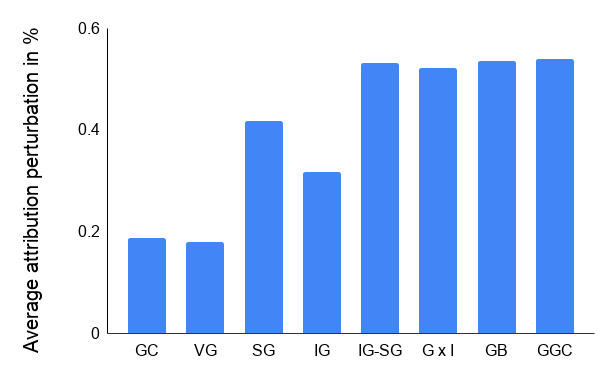
\includegraphics[width=.8\linewidth]{figures/ii_bar_raw.jpg}
  %\setlength\abovecaptionskip{-1ex}
  \setlength\belowcaptionskip{2ex}
  \caption{Average $g_c$ between $x$ and $x+\delta$ over 100 inputs.}
  \label{fig:ii_bar_raw}
\end{figure}


\section{DNN Architecture and training}
All BAM models are ResNet50~\cite{he2016deep} models. Training starts from an ImageNet pretrained checkpoint~\cite{Russakovsky15} (available at \url{https://github.com/tensorflow/models/tree/master/official/resnet}) and all layers are fine-tuned on the BAM dataset. 90\% of randomly chosen members of the BAM dataset are used to train, the rest are used for testing. All models are implemented using TensorFlow~\cite{abadi2016tensorflow} and trained on a single Nvidia Tesla V100 GPU. 

\section{Details of interpretability methods compared}

We consider neural network models with an input $x \in \mathbb{R}^d$ and a function $f(x): \mathbb{R}^d \mapsto \mathbb{R}^m$. A saliency method $e(f, x): \mathbb{R}^d \mapsto \mathbb{R}^d$ outputs a saliency map highlighting regions relevant to prediction. Below is an overview of the eight saliency methods evaluated in our work.

\textbf{GradCAM (GC)}~\cite{Selvaraju16} computes the gradient of the class logit with respect to the feature map of the last convolutional layer of a DNN. Guided GradCAM (GGC) is GC combined with Guided Backprop through an element-wise product.

\textbf{Vanilla Gradient (VG)}~\cite{Simonyan13,Erhan09,Baehrens10} computes the gradient of the target class $k$ at logit layer $l$ with respect to each input pixel: $e(f,x)=\frac{\partial f_l^k}{\partial x}$, reflecting how much the logit layer output would change when the input changes in a small neighborhood.

\textbf{SmoothGrad (SG)}~\cite{Smilkov17} reduces visual noise by averaging the explanations over a set of noisy images in the neighborhood of the original input image: $\frac{1}{|N|}\sum_{i=0}^N{e(f, x+z_i)}$, where $z_i \sim \mathcal{N}(\mu,\,\sigma^{2})$.

\textbf{Integrated Gradient (IG)}~\cite{Sundararajan17} computes the sum of gradients for a scaled set of images along the path between a baseline image ($x^\prime$) and the original input image: $e(f,x) = (x-x^\prime) \times \int_{0}^{1} \frac{\partial f(x^\prime + \alpha (x - x^\prime)}{\partial x}d\alpha$. Smoothing from SG can be applied to IG to produce IG-SG.

\textbf{Gradient x Input (G x I)} computes an element-wise product between VG and the original input image.~\cite{Ancona18} showed that for a ReLU network with zero baseline and no bias.

\textbf{Guided Backpropagation (GB)}~\cite{Springenberg14} builds on top of the DeConvNet explanation method~\cite{zeiler2014visualizing} and attributes input importance through backpropagating neuron activations from the logit layer to the input layer.

We accompany visualization of a subset of saliency methods by averaging over channels and capping the extremes to the $99^{th}$ percentile as done by~\cite{Sundararajan17,Smilkov17} before normalizing each attribution to between $[0,1]$. 

\section{Details of computing TCAV scores}
We compute the TCAV scores of the dog concept for different models (e.g. $f_o$ and $f_s$ for absolute contrast). To learn the dog CAV, we take 100 images from $X_{o,s}$ where the object is a dog as positive examples and 100 images from $X_{\varnothing,s}$ as negative examples for the dog concept. We perform two-sided t-test of the TCAV scores, and reject scores where $p$-value $>$ 0.01. We compute TCAV scores for each of the block layer and the logit layer of ResNet50. The final TCAV score is the average of the layers that passed statistical testing.

\section{Details of model contrast score baseline}
For model contrast score, we generate a random mask $I_c$ to calculate baseline differences. For TCAV, we obtain two TCAV scores for two models ($f_o$ and $f_s$), and show the difference between the two, both for TCAV scores for the dog CAVs and random CAVs. 

\section{Full size figures}%relative model contrast figures} 

\begin{figure*}
  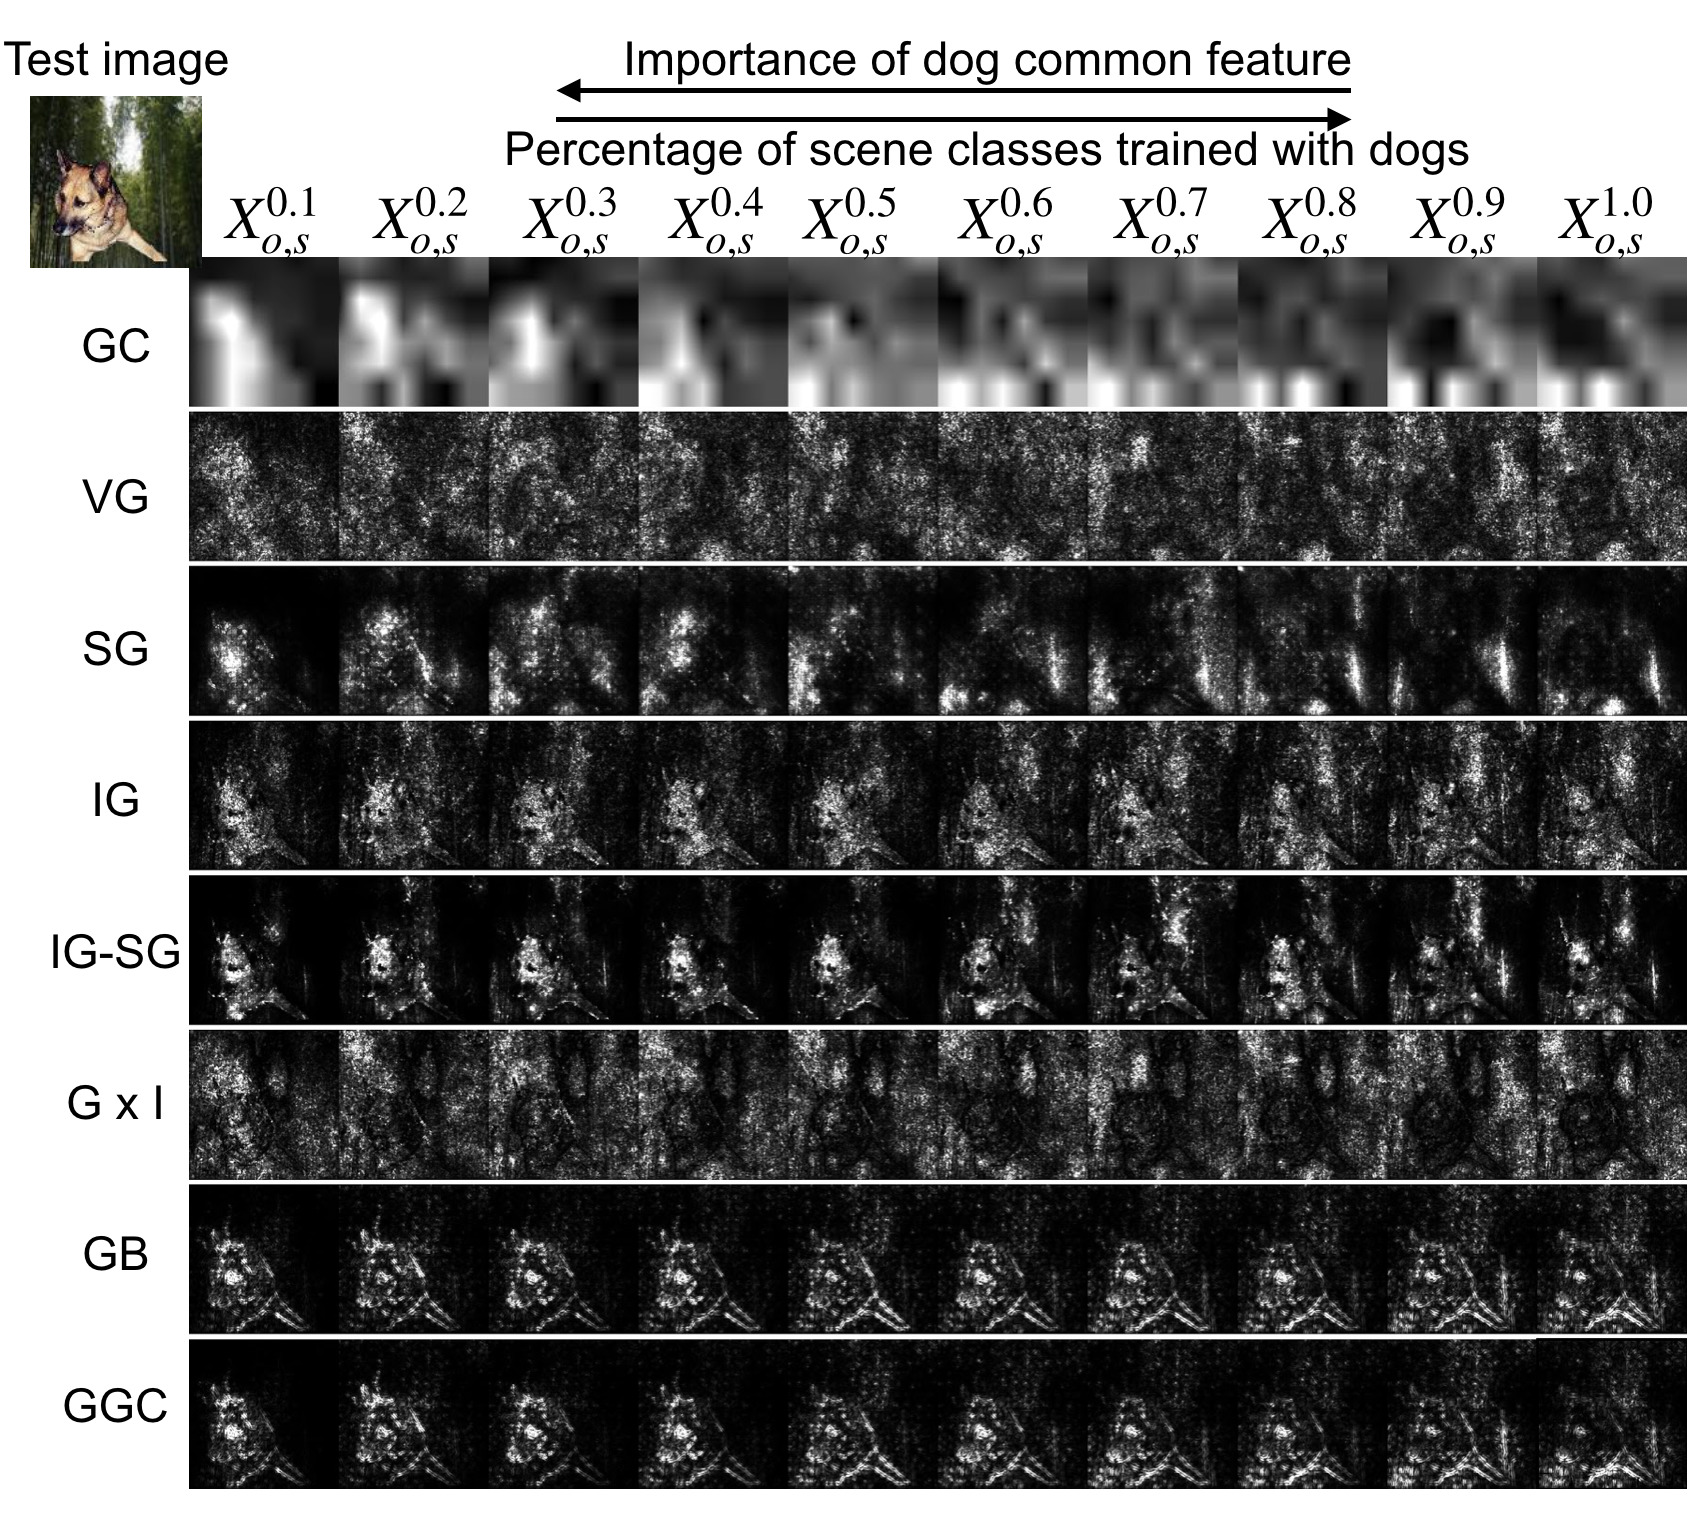
\includegraphics[width=1.\linewidth]{figures/rmc_demo.jpg}
  \caption{Full figure of an example of saliency map visualizations for models trained with \CF s of different $k$. $k$ increases from left to right. A larger contrast among each row is better.}
\end{figure*}
\begin{figure*}
  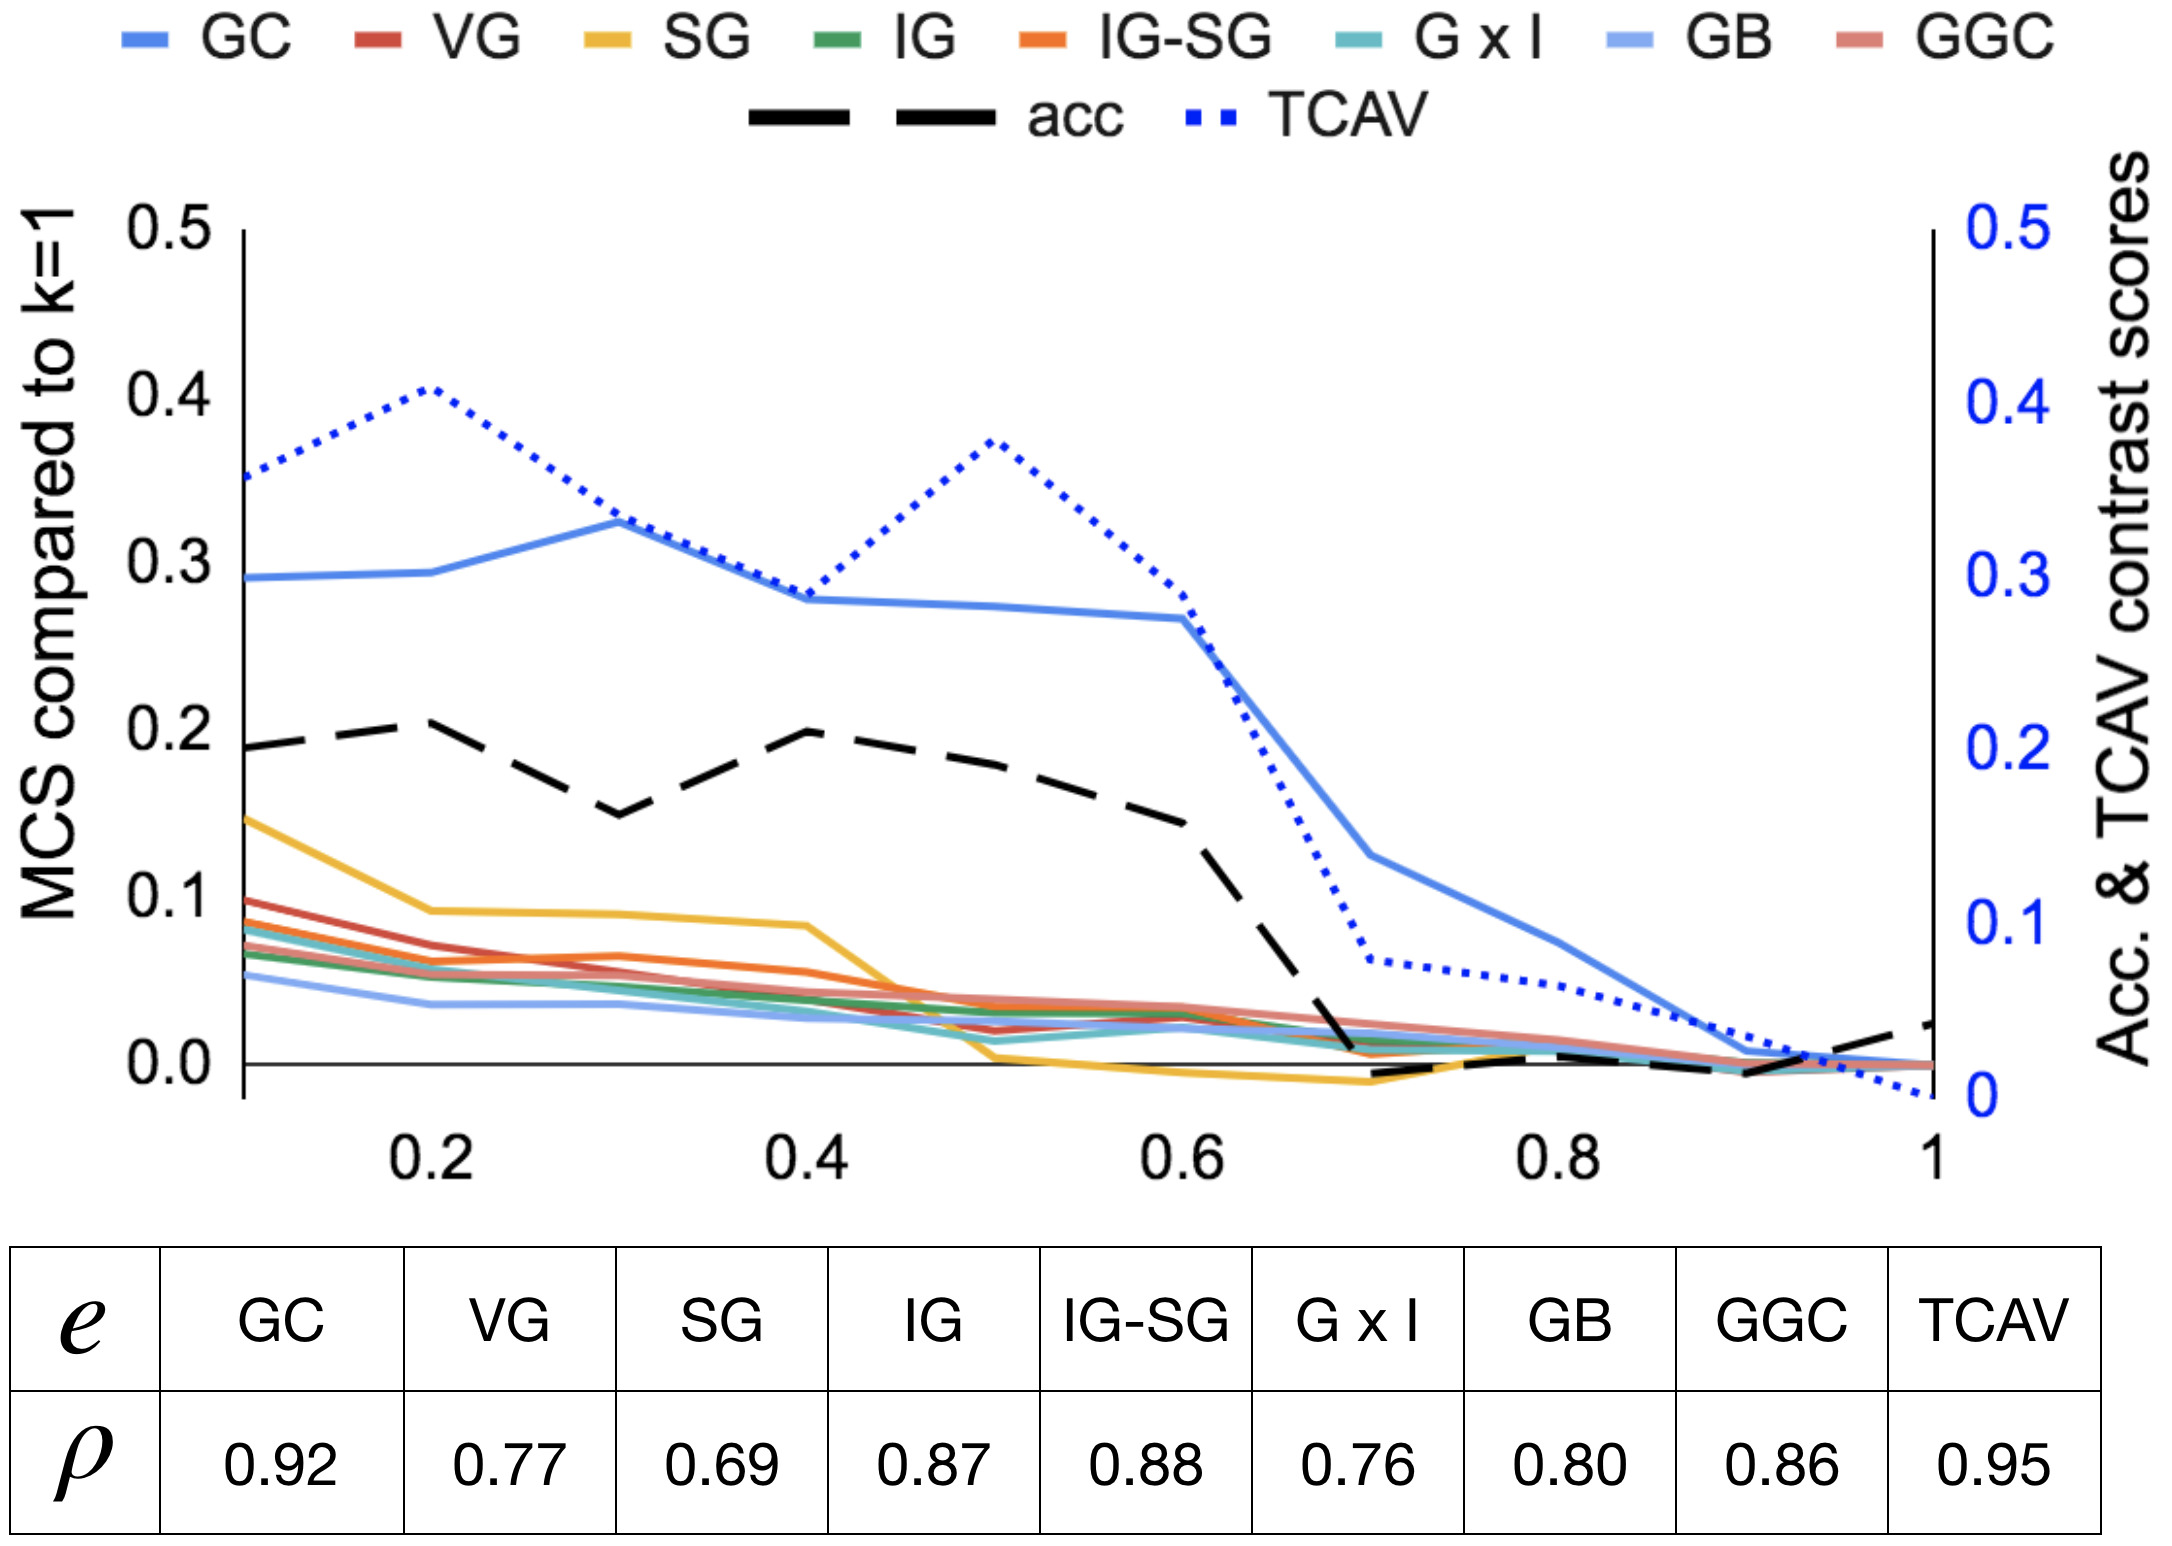
\includegraphics[width=1.\linewidth]{figures/rmc_chart.jpg}
  \caption{[Top] \MCS~between $\{X_{o,s}^k\}$ for $k \in \{0.1, \dots, 1.0\}$ and $X_{o,s}^{1.0}$ as $k$ increases. The dashed black line is the accuracy drop when \CF~is removed during testing. The dotted blue line is the series of \MCS~for TCAV. [Bottom] Pearson correlation coefficients ($\rho$) between each method's \MCS~and the accuracy drop. A higher correlation is better.}
\end{figure*}

\clearpage

%\section{Additional relative model contrast figures} 
\begin{figure*}[!]
  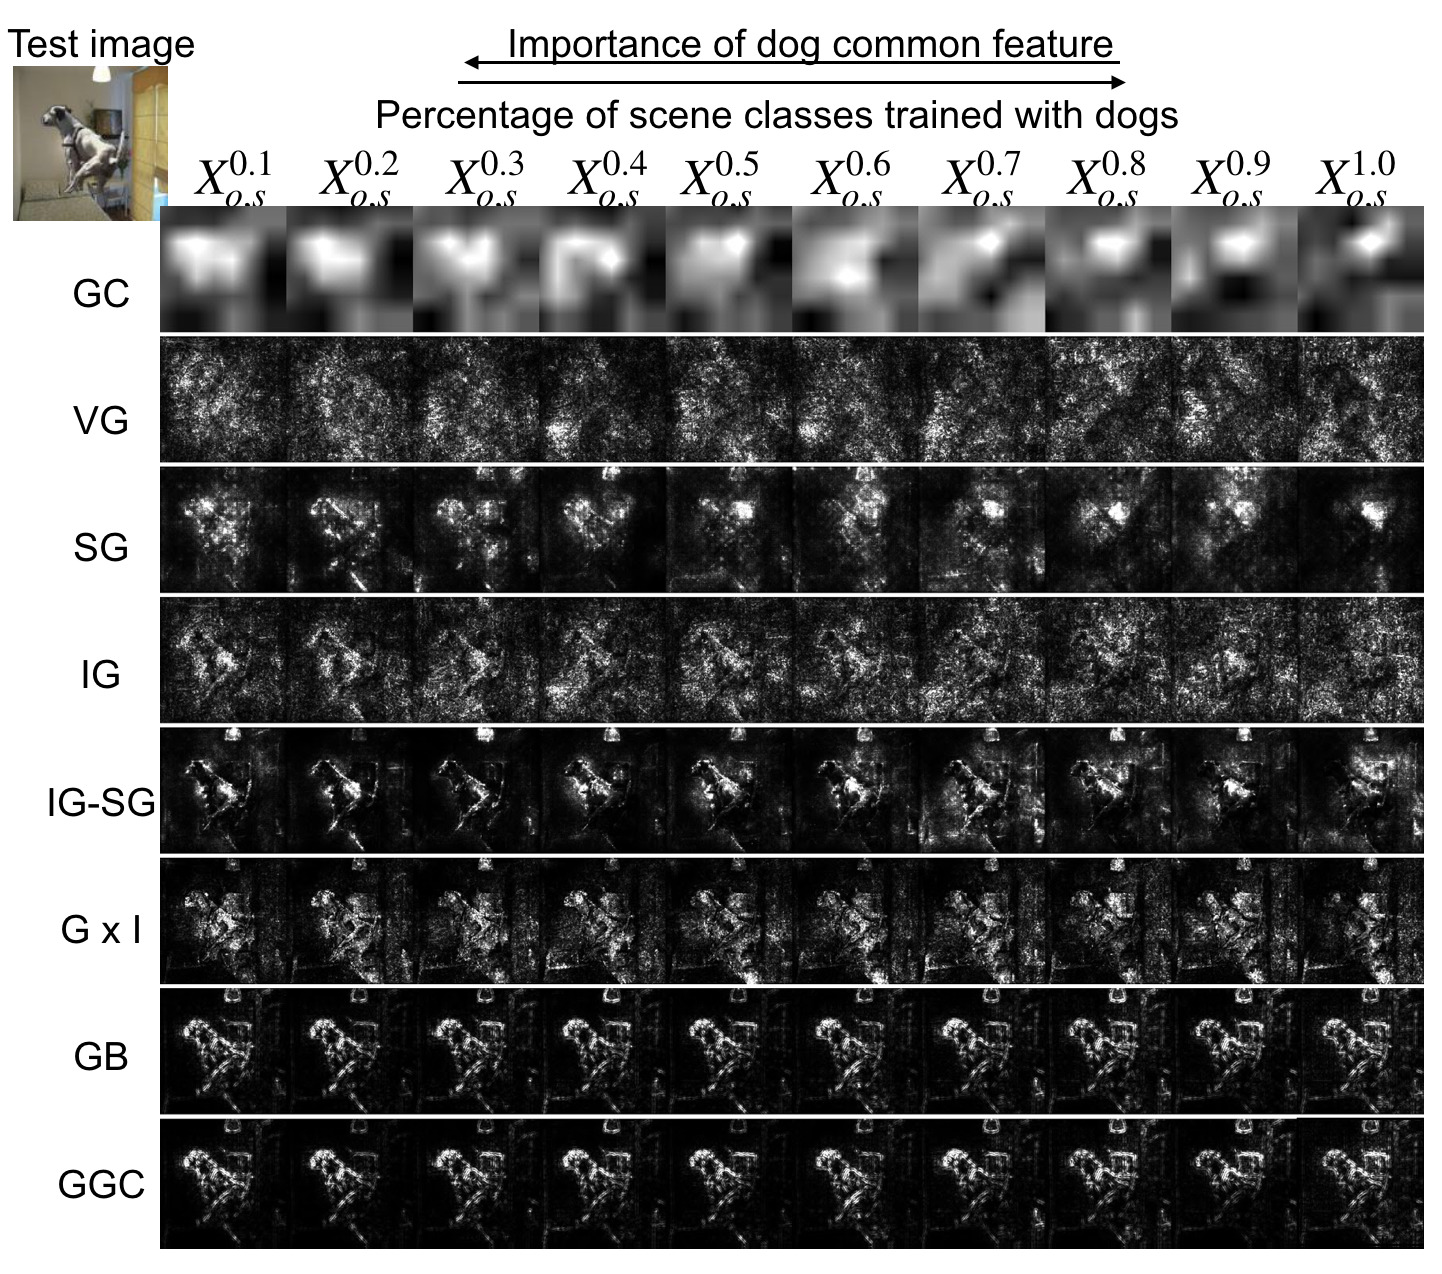
\includegraphics[width=1.\linewidth]{figures/rmc_demo28.jpg}
    \caption{Additional example saliency maps from relative model contrast testing.}
\end{figure*}
\begin{figure*}
  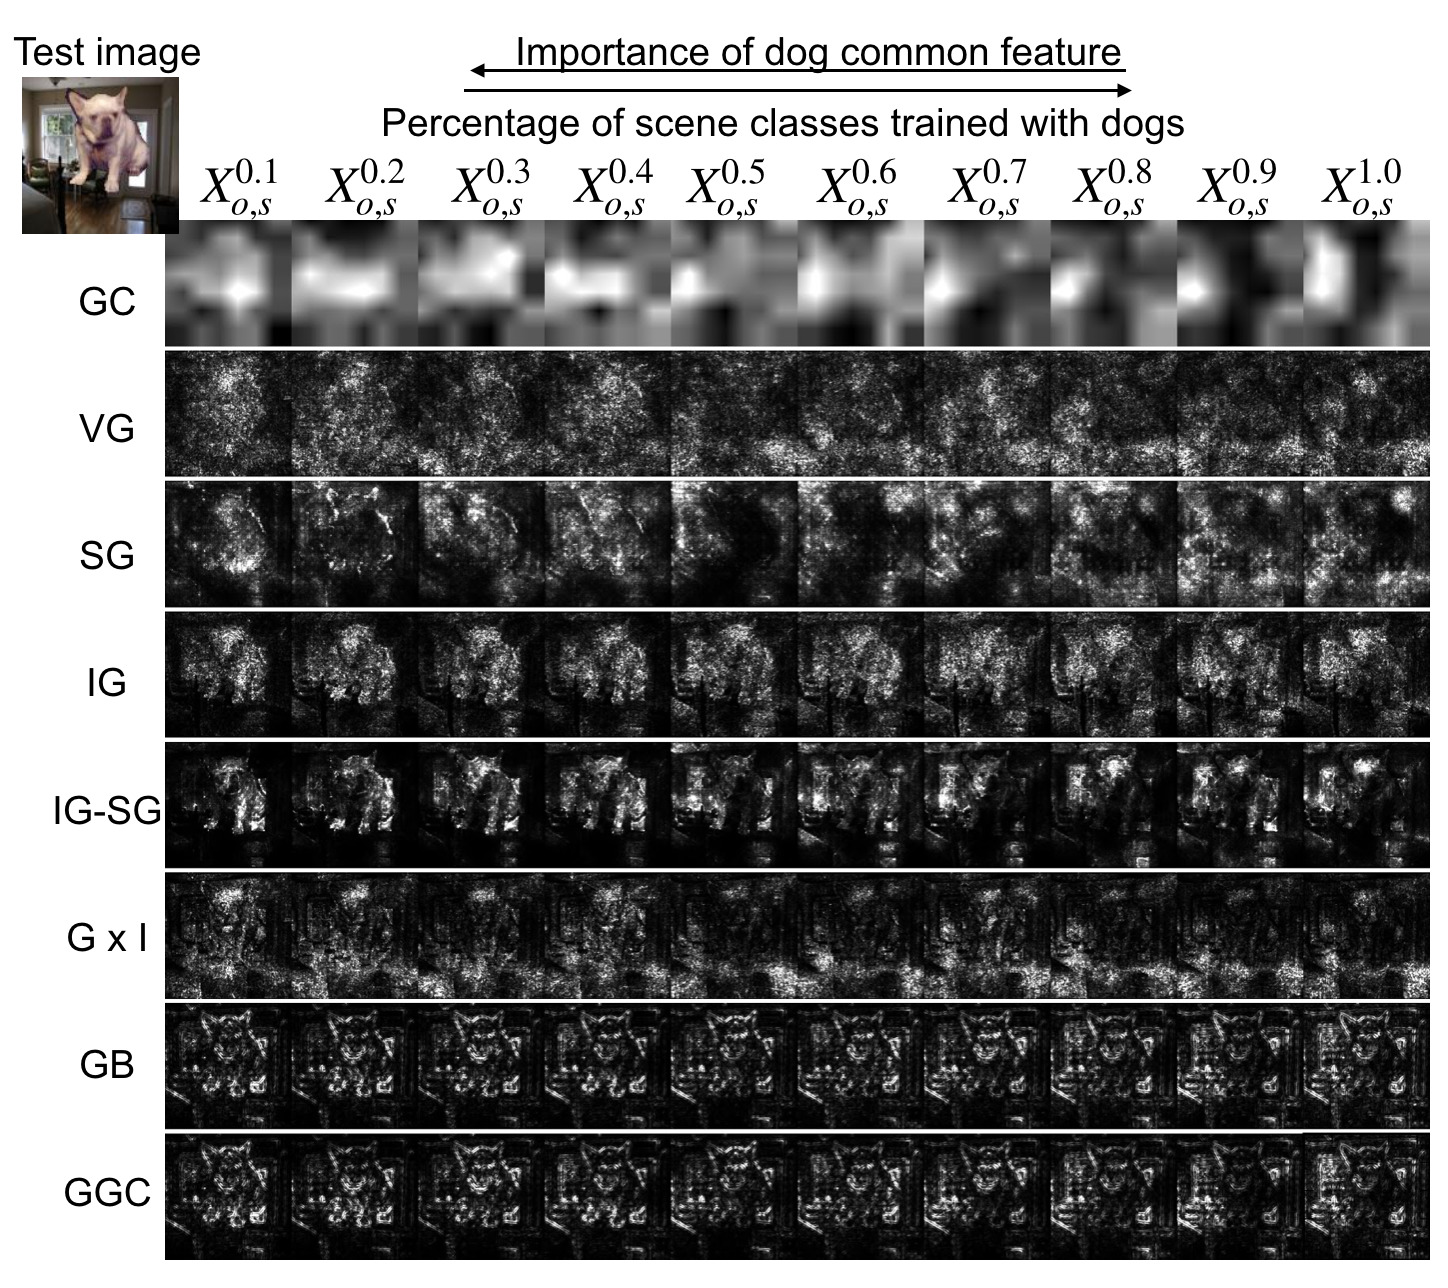
\includegraphics[width=1.\linewidth]{figures/rmc_demo58.jpg}
  \caption{Additional example saliency maps from relative model contrast testing.}
\end{figure*}

\clearpage

%\section{Additional input independence figures} 
\begin{figure*}
  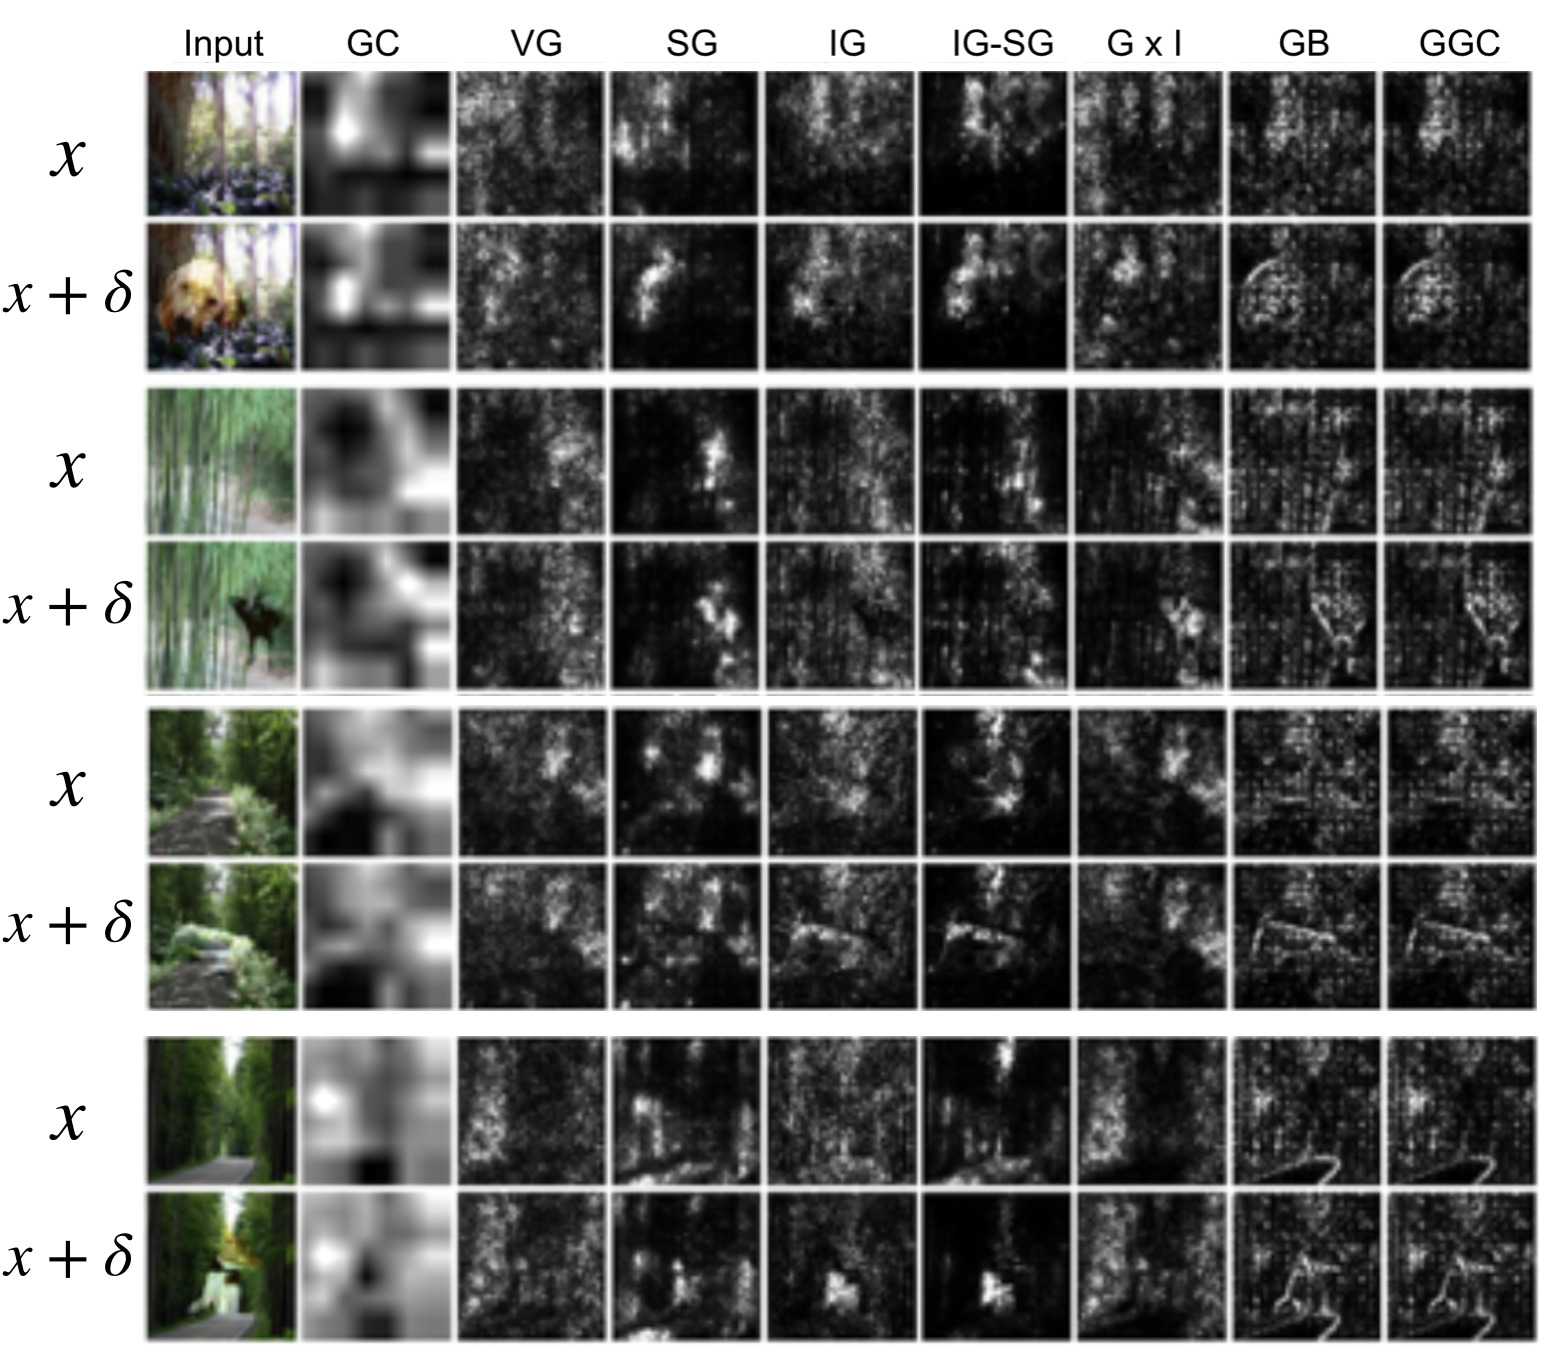
\includegraphics[width=1.\linewidth]{figures/ii_demo_extra.jpg}
  \caption{Additional example saliency maps from input independence testing.}
\end{figure*}

\end{appendix}